\documentclass[aspectratio=169, 10pt]{beamer}
\usepackage{fontspec}
\usepackage{xcolor}
\usepackage{tikz}
\usetikzlibrary{shapes.geometric, arrows.meta, positioning, calc, shadows}
\usepackage{pgfplots}
\pgfplotsset{compat=1.18}
\usepackage{tcolorbox}
\tcbuselibrary{skins}
\usepackage{graphicx}
\usepackage{booktabs}
\usepackage{hyperref}

% Define colors
\definecolor{mygreen}{HTML}{16A34A}
\definecolor{myred}{HTML}{DC2626}
\definecolor{mygray}{HTML}{475569}
\definecolor{mybg}{HTML}{F8FAFC}

% Beamer Theme
\usetheme{Boadilla}
\usecolortheme{default}
\setbeamercolor{structure}{fg=mygreen}
\setbeamercolor{palette primary}{bg=mygreen,fg=white}
\setbeamercolor{palette secondary}{bg=mygreen!80!black,fg=white}
\setbeamercolor{palette tertiary}{bg=mygreen!60!black,fg=white}
\setbeamercolor{titlelike}{fg=mygreen}
\setbeamercolor{item}{fg=mygreen}
\setbeamertemplate{itemize items}[circle]
\setbeamertemplate{navigation symbols}{}

\title{Dự đoán Sụp đổ Giá Cổ phiếu bằng\\ Suy luận Quan hệ theo Thời gian của LLM}
\subtitle{Đồ án Big Data $\cdot$ phỏng theo arXiv:2410.17266}
\author{Nhóm: [TÊN NHÓM] \\ Thành viên: [TÊN] \\ GVHD: [TÊN GV]}
\institute{Học kỳ / Năm}
\date{}

\begin{document}

\begin{frame}
    \titlepage
\end{frame}

\begin{frame}{Vấn đề \& Động lực}
    \begin{columns}
        \begin{column}{0.6\textwidth}
            \begin{itemize}
                \item Thị trường = dữ liệu \textbf{khối lượng lớn, tốc độ cao, đa dạng} $\rightarrow$ bài toán Big Data tiêu biểu.
                \item Dự đoán \textbf{hướng giá} (tăng/giảm) $\approx$ bất khả thi do thị trường hiệu quả dạng yếu (EMH).
                \item Nhưng \textbf{rủi ro sụp đổ (crash)} mang tín hiệu rõ từ TIN TỨC (tâm lý, sự kiện, lan truyền).
                \item \textbf{Mục tiêu:} Cảnh báo sớm rủi ro — Advisory cho nhà đầu tư / quản trị rủi ro (không phải lệnh mua–bán).
            \end{itemize}
        \end{column}
        \begin{column}{0.4\textwidth}
            \begin{tcolorbox}[colback=white, colframe=myred, title=Hướng giá (lên/xuống), fonttitle=\bfseries\small, boxrule=0.5mm]
                \centering $\approx$ Ngẫu nhiên (EMH)
            \end{tcolorbox}
            \vspace{0.2cm}
            \begin{tcolorbox}[colback=white, colframe=mygreen, title=Rủi ro sụp đổ (tail-risk), fonttitle=\bfseries\small, boxrule=0.5mm]
                \centering \checkmark Có tín hiệu từ tin tức
            \end{tcolorbox}
        \end{column}
    \end{columns}
\end{frame}

\begin{frame}{Bài toán (Định nghĩa chính xác)}
    \begin{itemize}
        \item \textbf{Đầu vào:} Dòng tin tài chính theo ngày cho 6 cổ phiếu: AAPL, AMZN, GOOGL, NVDA, TSLA, NFLX.
        \item \textbf{Đầu ra:} Xác suất $P(\text{danh mục equal-weight giảm} \ge 6\% \text{ trong 3 ngày tới})$ cho mỗi ngày.
        \item \textbf{Nhãn thực tế:} Từ giá lịch sử OHLCV (ngày gọi là crash nếu Low 3 ngày tới $\le -6\%$).
        \item \textbf{Đánh giá:} AUROC / PR-AUC. 
        \item \textbf{Nhân quả:} Chỉ dùng quá khứ (embargo $\ge$ tầm dự báo 3 ngày).
    \end{itemize}
    \vspace{0.5cm}
    \centering
    \begin{tikzpicture}[node distance=1.5cm, auto,
        box/.style={rectangle, draw, rounded corners, minimum height=1cm, align=center, fill=mybg, font=\small},
        arrow/.style={-{Stealth}, thick}]
        \node[box, draw=mygray] (news) {Tin ngày $t$};
        \node[box, draw=mygreen, right=of news] (model) {Mô hình TRR};
        \node[box, draw=mygreen, right=of model] (prob) {$P(\text{crash})$};
        \node[box, draw=myred, right=of prob] (label) {So sánh thực tế\\$\rightarrow$ Nhãn};
        
        \draw[arrow] (news) -- (model);
        \draw[arrow] (model) -- (prob);
        \draw[arrow] (prob) -- (label);
    \end{tikzpicture}
\end{frame}

\begin{frame}{Ý tưởng cốt lõi: LLM Suy Luận, Không Huấn Luyện}
    \begin{columns}
        \begin{column}{0.6\textwidth}
            \begin{itemize}
                \item Mô hình \textbf{zero-shot}: KHÔNG huấn luyện lại từ đầu — LLM trực tiếp \textbf{đọc và lập luận}.
                \item Phỏng theo khung TRR (Temporal Relational Reasoning).
                \item Chỉ sử dụng một \textbf{meta-learner nhỏ} học trên các đặc trưng dẫn xuất.
                \item Chuỗi \textbf{giá} lịch sử chỉ đóng vai trò cung cấp nhãn để đánh giá và filter.
            \end{itemize}
        \end{column}
        \begin{column}{0.4\textwidth}
            \centering
            \begin{tikzpicture}
                \node[align=center, text=myred, font=\bfseries] (no) {KHÔNG\\Train Model};
                \node[align=center, text=mygreen, font=\bfseries, right=1.5cm of no] (yes) {LLM SUY LUẬN\\Zero-shot};
                \node[font=\Large\bfseries, right=0.5cm of no] {$\neq$};
            \end{tikzpicture}
        \end{column}
    \end{columns}
\end{frame}

\begin{frame}{Phương pháp TRR: 4 Pha Xử Lý}
    \begin{enumerate}
        \item \textbf{Brainstorm:} Tin tức $\rightarrow$ Đồ thị tác động (VD: "X tác động $\pm$ lên Y").
        \item \textbf{Memory:} Bộ nhớ phân rã $R = \exp(-t\cdot\lambda)$ — ảnh hưởng của tin xấu nhạt dần theo thời gian.
        \item \textbf{Attention:} PageRank cắt tỉa đồ thị, chỉ giữ top-$k$ cạnh liên quan nhất đến danh mục.
        \item \textbf{Reason:} LLM suy luận trên đồ thị con $\rightarrow$ Trả về xác suất sụp đổ.
    \end{enumerate}
    \vspace{0.5cm}
    \centering
    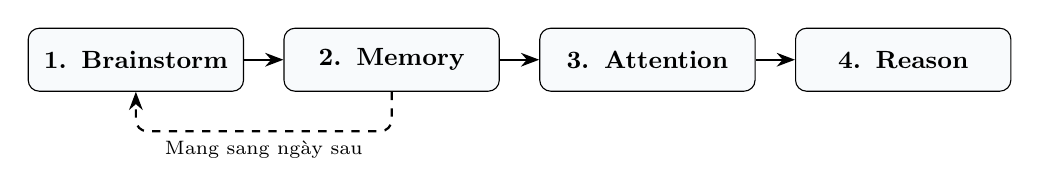
\begin{tikzpicture}[node distance=0.5cm, auto,
        box/.style={rectangle, draw, rounded corners, minimum height=0.8cm, text width=2.5cm, align=center, fill=mybg, font=\small\bfseries},
        arrow/.style={-{Stealth}, thick}]
        \node[box] (p1) {1. Brainstorm};
        \node[box, right=of p1] (p2) {2. Memory};
        \node[box, right=of p2] (p3) {3. Attention};
        \node[box, right=of p3] (p4) {4. Reason};
        
        \draw[arrow] (p1) -- (p2);
        \draw[arrow] (p2) -- (p3);
        \draw[arrow] (p3) -- (p4);
        \draw[arrow, dashed, rounded corners] (p2.south) -- +(0,-0.5) -| (p1.south) node[pos=0.25, below, font=\scriptsize] {Mang sang ngày sau};
    \end{tikzpicture}
\end{frame}

\begin{frame}{RAG: Truy hồi Tăng cường (Retrieval-Augmented Generation)}
    \begin{columns}
        \begin{column}{0.5\textwidth}
            \begin{tcolorbox}[title=Vai trò 1: Chọn lọc, colback=white, colframe=mygreen, boxrule=0.5mm]
                Từ kho tin khổng lồ mỗi ngày (hàng triệu bài), chỉ lấy $k$ tin \textbf{liên quan chặt chẽ} đến danh mục nhất $\rightarrow$ Giới hạn context cho LLM.
            \end{tcolorbox}
        \end{column}
        \begin{column}{0.5\textwidth}
            \begin{tcolorbox}[title=Vai trò 2: Few-shot theo tình huống, colback=white, colframe=mygreen, boxrule=0.5mm]
                Truy hồi các ngày quá khứ tương tự + kết cục thực tế ("đã crash" hoặc "không") và chèn vào prompt để LLM đối chiếu.
            \end{tcolorbox}
        \end{column}
    \end{columns}
    \vspace{0.3cm}
    \begin{itemize}
        \item \textbf{Kết quả:} Corpus dung lượng lớn nhưng \textbf{chi phí LLM vẫn $O(\text{số\_ngày} \times k)$}.
        \item Quá trình hoàn toàn tôn trọng tính nhân quả (chỉ nhìn về quá khứ).
    \end{itemize}
\end{frame}

\begin{frame}{Dữ liệu}
    \begin{columns}
        \begin{column}{0.45\textwidth}
            \begin{itemize}
                \item \textbf{FNSPID (Nguồn):} 23 GB thô, \textbf{15,7 triệu bài}, 4.775 mã cổ phiếu (1999–2023).
                \item \textbf{Corpus lọc (2016–2023):} \textbf{4,5 triệu bài / 12 GB}.
                \item \textbf{Giá OHLCV:} 6 mã, 2.012 ngày giao dịch (sinh nhãn crash).
                \item \textbf{Tin trực tiếp:} $\sim$500 tin/ngày (từ yfinance \& Google News RSS).
            \end{itemize}
        \end{column}
        \begin{column}{0.55\textwidth}
            \centering
            \begin{tikzpicture}[scale=0.7]
                \begin{axis}[
                    ybar,
                    bar width=15pt,
                    enlarge x limits=0.15,
                    ylabel={Số bài (Nghìn)},
                    symbolic x coords={2016,2017,2018,2019,2020,2021,2022,2023},
                    xtick=data,
                    nodes near coords,
                    nodes near coords align={vertical},
                    ymin=0, ymax=1100,
                    width=\textwidth,
                    height=6cm,
                    title={\textbf{Số bài tin trong corpus (Tổng 4,5 triệu)}},
                    ]
                    \addplot[fill=mygreen!80, draw=none] coordinates {
                        (2016,818) (2017,516) (2018,699) (2019,700) 
                        (2020,352) (2021,182) (2022,280) (2023,954)
                    };
                \end{axis}
            \end{tikzpicture}
        \end{column}
    \end{columns}
\end{frame}

\begin{frame}{Bốn chữ V của Big Data}
    \begin{columns}
        \begin{column}{0.5\textwidth}
            \begin{tcolorbox}[title=Volume (Khối lượng), colback=white, colframe=mygray, boxrule=0.5mm]
                23 GB / 15,7 triệu bài thô\\$\rightarrow$ 12 GB / 4,5 triệu bài sau lọc.
            \end{tcolorbox}
            \vspace{0.1cm}
            \begin{tcolorbox}[title=Velocity (Tốc độ), colback=white, colframe=mygray, boxrule=0.5mm]
                Luồng trực tiếp $\sim$500 tin/ngày,\\Cập nhật mỗi 60 giây (Spark Streaming).
            \end{tcolorbox}
        \end{column}
        \begin{column}{0.5\textwidth}
            \begin{tcolorbox}[title=Variety (Đa dạng), colback=white, colframe=mygray, boxrule=0.5mm]
                Tin công ty, vĩ mô, crypto, thế giới; Dữ liệu giá (nhiều nguồn phi cấu trúc \& cấu trúc).
            \end{tcolorbox}
            \vspace{0.1cm}
            \begin{tcolorbox}[title=Value (Giá trị), colback=white, colframe=mygray, boxrule=0.5mm]
                Advisory cảnh báo sụp đổ danh mục + Web app triển khai thực tế.
            \end{tcolorbox}
        \end{column}
    \end{columns}
\end{frame}

\begin{frame}{Kiến trúc Lưu trữ: "Lưu khổng lồ, phục vụ tí hon"}
    \begin{itemize}
        \item \textbf{Lạnh:} Corpus 12 GB lưu trữ trên đĩa cứng.
        \item \textbf{Ấm:} SQLite chỉ mục theo ngày (1,9 GB) cho phép tra cứu 1 ngày trong $\sim$44 ms.
        \item \textbf{Nóng:} Lát dữ liệu RAG đã lọc để đưa vào LLM chỉ $\sim$2 MB.
    \end{itemize}
    \vspace{0.3cm}
    \textbf{Kỹ thuật tối ưu:}
    \begin{itemize}
        \item Stream-and-filter: Không nạp toàn bộ 23 GB thô vào RAM.
        \item Chỉ định dạng cột cần thiết và sử dụng chỉ mục phân vùng.
        \item \textbf{Nguyên tắc:} Dữ liệu dẫn xuất không commit vào Git, chỉ commit code tái tạo (Reproducibility).
    \end{itemize}
\end{frame}

\begin{frame}{Xử lý Phân tán: Apache Spark}
    \begin{columns}
        \begin{column}{0.55\textwidth}
            \begin{itemize}
                \item \textbf{Spark ETL:} Chuyển corpus 12 GB sang định dạng \textbf{Parquet phân vùng theo năm} (chuẩn Data-lake/HDFS).
                \item Đo lường thực tế:
                \begin{itemize}
                    \item Chuyển đổi 12 GB CSV $\rightarrow$ \textbf{718 MB Parquet} trong 101 giây.
                    \item Truy vấn \textbf{4,5 triệu dòng} từ Parquet mất \textbf{2,4 giây} (nhanh hơn $\sim$40$\times$, 8 lõi song song).
                    \item \textbf{Partition pruning:} Quét riêng năm 2020 chỉ mất \textbf{0,2 giây}.
                \end{itemize}
                \item Cùng source code có thể chạy cluster thực tế (đổi \texttt{SPARK\_MASTER}).
            \end{itemize}
        \end{column}
        \begin{column}{0.45\textwidth}
            \centering
            \begin{tikzpicture}[scale=0.7]
                \begin{axis}[
                    xbar,
                    y dir=reverse,
                    bar width=15pt,
                    enlarge y limits=0.5,
                    xlabel={Thời gian quét (giây)},
                    ytick={1,2},
                    yticklabels={Đọc CSV (1 lõi), Đọc Parquet (8 lõi)},
                    nodes near coords,
                    nodes near coords align={horizontal},
                    xmin=0, xmax=120,
                    width=\textwidth,
                    height=4cm,
                    title={\textbf{Tốc độ truy vấn 4,5 triệu dòng}},
                    ]
                    \addplot[fill=mygreen!80, draw=none] coordinates {
                        (101,1) (2.4,2)
                    };
                \end{axis}
            \end{tikzpicture}
        \end{column}
    \end{columns}
\end{frame}

\begin{frame}{Tính toán Phân tán: Fan-out GPU}
    \begin{itemize}
        \item \textbf{Điểm nghẽn:} Suy luận của mô hình LLM 32B rất nặng.
        \item \textbf{Giải pháp:} Phân tán thành \textbf{40 mảnh (shard)} (20 base + 20 RAG) chạy song song độc lập.
        \item Chạy trên một \textbf{pool GPU Kaggle} $\rightarrow$ Hoàn thành cả 40 mảnh trong \textbf{$\sim$20 phút} thay vì $\sim$5 giờ (tuần tự).
        \item Mỗi shard bao gồm $\sim$101 ngày và một \textbf{kho ngày lịch sử đầy đủ} để giữ tính nhân quả (lookback).
        \item \textbf{Lưu ý:} Phân tán ở đây chỉ giúp \textbf{TĂNG TỐC}, chạy 1 máy tuần tự vẫn cho KẾT QUẢ Y HỆT.
    \end{itemize}
\end{frame}

\begin{frame}{Mô hình \& Triển khai}
    \begin{itemize}
        \item \textbf{Offline Backtest (Quy mô lớn):} Dùng \textbf{Qwen2.5-32B} (Kaggle RTX 6000 Pro) để đánh giá.
        \item \textbf{Suy luận trực tiếp (Live):} Dùng \textbf{Qwen2.5-7B-AWQ} (RTX 2060 SUPER 8 GB cục bộ) cho dự đoán thời gian thực.
        \item \textbf{Hệ thống:}
        \begin{itemize}
            \item \textbf{FastAPI:} Các endpoint \texttt{/predict}, \texttt{/predict-ensemble}, \texttt{/backtest}.
            \item \textbf{Streamlit Web App:} Giao diện giám sát trực tiếp, nạp $\sim$500 tin/ngày và biểu đồ tương tác.
            \item \textbf{Daemon background:} Crawl và cập nhật mỗi 60 giây, lưu rolling 7 ngày.
        \end{itemize}
    \end{itemize}
\end{frame}

\begin{frame}{Hiển thị $\neq$ Dự đoán}
    \begin{columns}
        \begin{column}{0.5\textwidth}
            \begin{itemize}
                \item Giao diện Web hiển thị 4 nhóm tin: Công ty, Vĩ mô, Crypto, Thế giới.
                \item \textbf{Dự đoán mô hình CHỈ DÙNG:} Tin Công ty + Vĩ mô (khớp với phân phối dữ liệu đã huấn luyện).
                \item Các tin Crypto / Thế giới bị \textbf{loại bỏ} hoàn toàn trước khi đi vào LLM suy luận.
                \item Feed trực tiếp \textbf{không có nhãn đánh giá} $\rightarrow$ mục đích để \textbf{chứng minh khả năng triển khai thực tế}.
            \end{itemize}
        \end{column}
        \begin{column}{0.5\textwidth}
            \centering
            \begin{tikzpicture}[box/.style={rectangle, draw, rounded corners, fill=mybg, minimum width=2.5cm, align=center, font=\small},
                arrow/.style={-{Stealth}, thick}]
                \node[box] (all) {Công ty\\Vĩ mô\\Crypto\\Thế giới};
                \node[box, right=2cm of all, fill=mygreen!20, draw=mygreen, thick] (predict) {LLM Dự đoán\\(Công ty + Vĩ mô)};
                \node[box, below=1cm of predict, fill=mygray!20, draw=mygray, text=mygray, thick] (display) {Chỉ Hiển thị\\(Crypto + Thế giới)};
                
                \draw[arrow] (all.east) -- ++(0.8,0) |- (predict.west);
                \draw[arrow, color=mygray] (all.east) -- ++(0.8,0) |- (display.west);
            \end{tikzpicture}
        \end{column}
    \end{columns}
\end{frame}

\begin{frame}{Kết quả (1): Số đã có}
    \begin{columns}
        \begin{column}{0.4\textwidth}
            \begin{itemize}
                \item \textbf{Cửa sổ COVID} (2019–2020):
                \begin{itemize}
                    \item Base: \textbf{0.785}
                    \item +RAG: \textbf{0.847}
                \end{itemize}
                \item \textbf{Cửa sổ rộng} (2016–2020):
                \begin{itemize}
                    \item Base: \textbf{0.710}
                    \item +RAG: tăng \textbf{0.074} (\textit{p=0.009}, có ý nghĩa thống kê).
                \end{itemize}
                \item \textbf{Baseline (Khối lượng tin):} $\approx 0.50$ (Ngẫu nhiên) $\rightarrow$ Tín hiệu dự đoán đến từ \textbf{suy luận ngữ nghĩa}, không phải đếm số lượng.
            \end{itemize}
        \end{column}
        \begin{column}{0.6\textwidth}
            \centering
            \begin{tikzpicture}[scale=0.8]
                \begin{axis}[
                    ybar,
                    bar width=20pt,
                    enlarge x limits=0.4,
                    ylabel={AUROC},
                    xtick={1,2},
                    xticklabels={COVID (2019-2020), Rộng (2016-2020)},
                    nodes near coords,
                    nodes near coords align={vertical},
                    ymin=0.4, ymax=0.95,
                    width=\textwidth,
                    height=6cm,
                    legend style={at={(0.5,-0.15)}, anchor=north, legend columns=-1},
                    ]
                    \addplot[fill=mygray!50, draw=none] coordinates {(1,0.785) (2,0.710)};
                    \addplot[fill=mygreen!80, draw=none] coordinates {(1,0.847) (2,0.784)};
                    \legend{Base (Không RAG), +RAG}
                    \draw[red, dashed, thick] (axis cs:1,0.5) -- (axis cs:2,0.5) node[pos=0.5, above] {0.50 (Ngẫu nhiên)};
                \end{axis}
            \end{tikzpicture}
        \end{column}
    \end{columns}
\end{frame}

\begin{frame}{Kết quả (2): Mở rộng Toàn bộ Corpus 2016–2023}
    \begin{columns}
        \begin{column}{0.5\textwidth}
            \textbf{So sánh trên CÙNG cửa sổ:}
            \begin{itemize}
                \item \textbf{COVID:} Base \textbf{0.707} / RAG \textbf{0.763} \textit{(Cũ: 0.847)}
                \item \textbf{2016–2020:} Base \textbf{0.693} / RAG \textbf{0.681} \textit{(Cũ: 0.710)}
                \item \textbf{Toàn bộ 2016–2023:} Base \textbf{0.615} / RAG \textbf{0.652}
            \end{itemize}
            \vspace{0.3cm}
            \textbf{Kết luận:}
            \begin{itemize}
                \item Lọc theo danh mục giúp \textbf{hồi phục mạnh} (từ 0.37 lên 0.76 trong tập COVID).
                \item Tuy nhiên, sử dụng corpus lớn \textbf{không vượt qua} bộ dữ liệu gộp gốc.
                \item \textbf{Bài học:} Trong phân tích tin tức tài chính, \textit{nhiều dữ liệu hơn không đồng nghĩa với kết quả tốt hơn}.
            \end{itemize}
        \end{column}
        \begin{column}{0.5\textwidth}
            \centering
            \begin{tikzpicture}[scale=0.75]
                \begin{axis}[
                    ybar,
                    bar width=15pt,
                    enlarge x limits=0.25,
                    ylabel={AUROC},
                    xtick={1,2,3},
                    xticklabels={COVID, 2016-2020, Toàn bộ 23},
                    nodes near coords,
                    nodes near coords align={vertical},
                    ymin=0.4, ymax=0.9,
                    width=\textwidth,
                    height=6cm,
                    legend style={at={(0.5,-0.15)}, anchor=north, legend columns=-1},
                    ]
                    \addplot[fill=mygray!50, draw=none] coordinates {(1,0.707) (2,0.693) (3,0.615)};
                    \addplot[fill=mygreen!80, draw=none] coordinates {(1,0.763) (2,0.681) (3,0.652)};
                    \legend{Base, RAG}
                    \draw[red, dashed, thick] (axis cs:1,0.5) -- (axis cs:3,0.5);
                \end{axis}
            \end{tikzpicture}
        \end{column}
    \end{columns}
\end{frame}

\begin{frame}{Phân tích Trung thực (Honest Analysis)}
    \begin{table}[]
        \centering
        \renewcommand{\arraystretch}{1.3}
        \begin{tabular}{p{0.45\textwidth} p{0.45\textwidth}}
            \toprule
            \textbf{\textcolor{mygreen}{Điều đã hoạt động tốt \checkmark}} & \textbf{\textcolor{myred}{Giới hạn / Kết quả âm $\times$}} \\ \midrule
            \textbf{RAG ổn định:} Cải thiện dự đoán trong khủng hoảng (COVID). & \textbf{Small-N:} Chỉ có 14–82 ngày crash ($\sim 4\%$), điểm AUROC tuyệt đối cần được đọc thận trọng. \\ 
            \textbf{Kiến trúc Big Data:} Stream-index-select, Spark ETL + Parquet hiệu quả cao. & \textbf{Các thử nghiệm thất bại:} Graph-RAG đa bước, mạng hướng 3 lớp, đặc trưng OHLCV Volume không tăng hiệu suất. \\ 
            \textbf{Phân tán Fan-out:} Tối ưu hóa được điểm nghẽn GPU bằng pool Kaggle free-tier. & \textbf{Bẫy Big Data:} Corpus toàn mã làm giảm mạnh tín hiệu (liên quan $\neq$ liên quan danh mục). \\ 
            \bottomrule
        \end{tabular}
    \end{table}
\end{frame}

\begin{frame}{Kết luận \& Hướng phát triển}
    \begin{itemize}
        \item \textbf{Đóng góp chính:}
        \begin{enumerate}
            \item Áp dụng thành công mô hình \textbf{TRR Zero-shot + RAG} để dự đoán rủi ro sụp đổ chứng khoán từ tin tức văn bản.
            \item \textbf{Kiến trúc RAG} chứng minh được sự cải thiện ổn định trong các cửa sổ khủng hoảng.
            \item Triển khai \textbf{hạ tầng Big Data thực tế}: xử lý luồng tin 23 GB bằng kỹ thuật Stream-Index-Select, lưu trữ Parquet qua Spark và phân tán inference bằng pool GPU.
        \end{enumerate}
        \vspace{0.4cm}
        \item \textbf{Hướng phát triển trong tương lai:}
        \begin{itemize}
            \item Mở rộng sang cluster Spark/HDFS phân tán trên nhiều máy vật lý thực tế.
            \item Tích hợp corpus đa nguồn (Mạng xã hội, Báo cáo tài chính).
            \item Hiệu chỉnh ngưỡng xác suất theo bài toán chi phí rủi ro và mở rộng dự đoán đa tài sản.
        \end{itemize}
    \end{itemize}
\end{frame}

\begin{frame}[plain]
    \centering
    \vspace{2cm}
    \Huge \textbf{\textcolor{mygreen}{Cảm ơn thầy/cô và các bạn đã lắng nghe!}}
    
    \vspace{1.5cm}
    \Large \textbf{Q\&A}
    
    \vspace{1.5cm}
    \normalsize \textbf{Mã nguồn Đồ án:} \\
    \url{https://github.com/duongtrongnguyen123/bigdata-stock-crash-trr}
\end{frame}

\end{document}
